\section{Implementación, interfaz y documentación}

\subsection{Implementación}

\subsubsection{Carga y validación de datos}

La instancia se carga desde los siete archivos CSV de \texttt{data/}. La
implementación utiliza \texttt{pandas} para leer las tablas y
\texttt{PuLP} para construir el modelo entero. El archivo
\texttt{modelo.py}, dentro de \texttt{2\_implementacion/}, separa la carga y validación de los datos
de la construcción y resolución del modelo.

Antes de resolver se comprueban los encabezados obligatorios, los identificadores
duplicados, los valores numéricos y las relaciones entre actividades y espacios.
También se valida que el horizonte y las franjas por día formen un número entero
de días. Los errores de estructura o referencia se presentan como errores de
datos.

\subsubsection{Construcción y resolución}

La formulación se representa con variables binarias \texttt{y[i]} para la
selección y \texttt{x[i,e,t]} para la asignación inicial. Solo se crean variables
factibles desde el punto de vista de compatibilidad, capacidad, disponibilidad y
duración.

Las restricciones se aplican sobre cada franja: el presupuesto suma los costes
de las actividades seleccionadas y las actividades obligatorias toman el valor
uno. La ocupación impide solapes dentro de un espacio, también para actividades
de varias franjas. La ampliación impide que los pares incompatibles ocupen la
misma franja.

La función objetivo combina la asistencia, la valoración y el número de
actividades. La interfaz permite fijar los pesos de asistencia y valoración y
calcula \(w_N=1-w_A-w_V\), de modo que los pesos efectivos cumplen
\(w_A+w_V+w_N=1\). Como defensa adicional, el motor normaliza una terna recibida
desde código y rechaza una terna totalmente nula. El modelo se resuelve con el
solver HiGHS mediante \texttt{pulp.HiGHS}. La implementación distingue solución
óptima, problema inviable y error del solver o de los datos.

\subsection{Interfaz}

\subsubsection{Configuración y ejecución}

La interfaz se desarrolla con Streamlit en \texttt{streamlit\_app.py}. Permite
modificar el presupuesto y los pesos de asistencia y valoración. El peso del
número de actividades se calcula como \(w_N=1-w_A-w_V\), por lo que los tres
pesos siempre suman uno. La interfaz muestra además la terna efectiva y su suma.
Al pulsar el botón de resolución se indica si existe una solución óptima, si el
problema es inviable o si se ha producido un error.

\subsubsection{Presentación de resultados}

Para una solución óptima, la interfaz presenta el número de actividades,
asistencia, valoración, coste y presupuesto. También muestra un calendario
ordenado por espacios y franjas, identificado con etiquetas como \texttt{D1F3},
y una tabla con las actividades seleccionadas.

La tabla detallada conserva la actividad, categoría, duración, asistencia,
valoración, coste, espacio y franjas inicial y final. Permite comprobar la
asignación sin gráficos complejos. La interfaz carga la instancia principal
desde \texttt{data/} y ofrece la descarga CSV integrada de esta tabla de
actividades seleccionadas. Al mantener los archivos de entrada separados del
código, se puede modificar la instancia y ejecutar otra resolución compatible.

Las actividades no seleccionadas se muestran de forma compacta en una sección
plegable, para cumplir el requisito de informar de los descartes sin sobrecargar
la vista principal.

\begin{figure}[htbp]
\centering
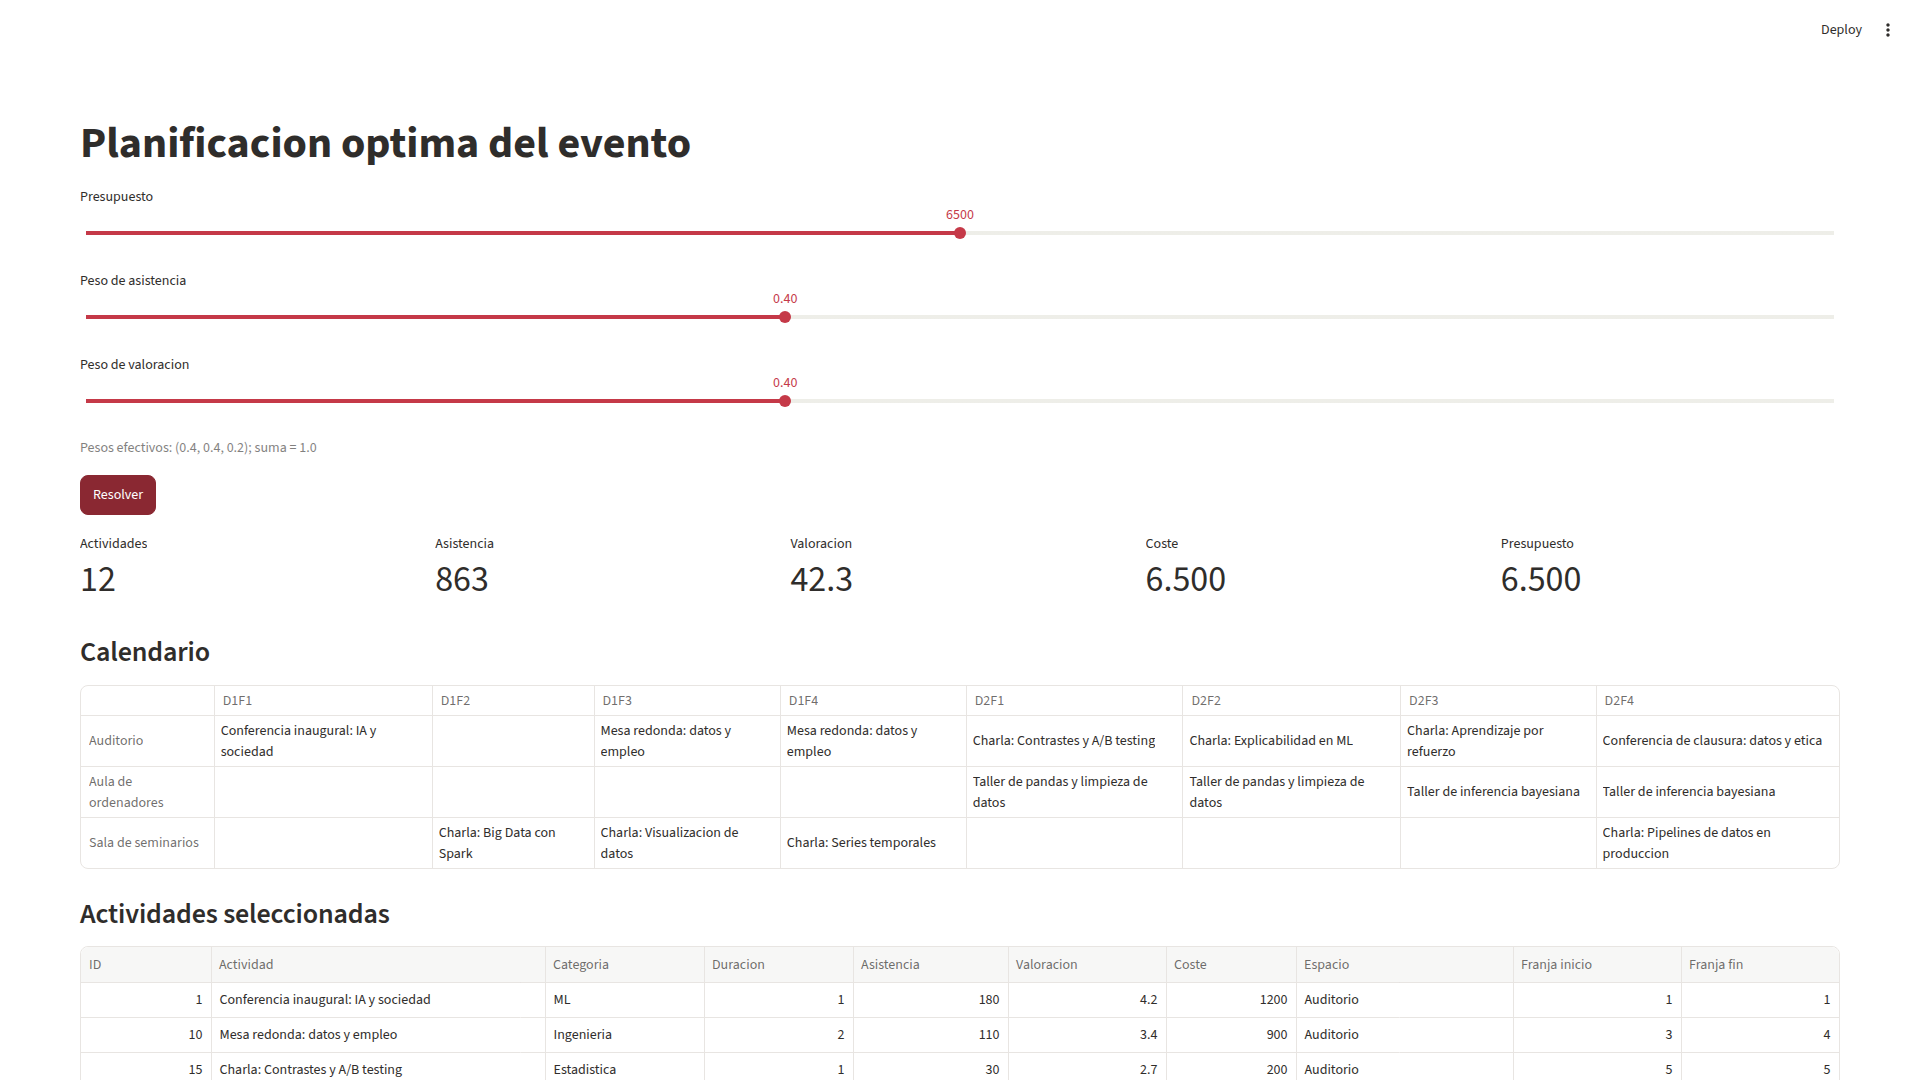
\includegraphics[width=\textwidth]{../images/ss.png}
\caption{Interfaz de Streamlit y resultados de una resolución.}
\label{fig:interfaz}
\end{figure}

\subsection{Documentación}

\subsubsection{Dependencias y ejecución}

Las dependencias se documentan en \texttt{requirements.txt} e incluyen
\texttt{streamlit}, \texttt{pandas}, \texttt{PuLP} y \texttt{highspy}. El
\texttt{README.md} indica la creación del entorno virtual, la instalación y la
ejecución local mediante \texttt{python -m streamlit run streamlit\_app.py}.
